\chapter{Neuronowa sieć konwolucyjna}
\label{chap:cnn}
\section{Wstęp}
\label{cnn-wstęp}
W przypadku zagadnień z dziedziny analizy obrazu, same sieci gęste robią się niepraktyczne. Teoretycznie możliwe jest przetworzenie obrazu w taki sposób, że każdy piksel traktowany jest jako jeden węzeł sieci,
ale już przy obrazkach o wymiarach 100x100x3 (100 na 100 pikseli, 3 kanały RGB) daje to 30000 węzłów na warstwie pierwszej. Nawet gdyby warstwa druga
miała być dwa razy mniejsza tj. 15000 węzłów macierz \(w^{\lbrack 1\rbrack}\) miałaby wymiar (30000, 15000). 
Przy założeniu, że rozmiar liczby typu double to 64 bity, to sama taka pojedyncza macierz miałaby rozmiar \(64\) \lbrack b\rbrack \(\times 30000 \times 15000 \times \frac{1}{8\ }\ \times \frac{1}{1024\ } \times \frac{1}{1024\ }\  \approx \ 3433\ \)\lbrack MB\rbrack. Poza problemami z pamięcią,
leży wziąć pod uwagę wysoki koszt obliczeniowy operacji na tak dużych macierzach, a przecież rozdzielczość współczesnych obrazów jest wielokrotnie wyższa. By poradzić sobie z tym problemem, należało wprowadzić inny rodzaj architektury sieci neuronowej -- konwolucyjną sieć neuronową (ang. \textit{convolutional neural network}, w skrócie \textit{CNN}).

\section{Opis elementów składających się na konwolucyjną sieć neuronową}
\label{opis-elementów-cnn}

\subsection{Filtry i splot w konwolucyjnej sieci neuronowej}

By ograniczyć liczbę węzłów, definiuje się tzw. filtry. Są to macierze kwadratowe, wypełnione wagami \(w\) których wartość jest ustalana w procesie propagacji wstecznej. Macierze te są układane w warstwy a liczba tych warstw determinowana jest przez liczba kanałów obrazu wejściowego lub poprzedniej warstwy sieci konwolucyjnej.

By uzyskać wynik, stosuje się na obrazie dyskretną operację splotu z filtrem lub filtrami. Taka operacja wykonywana jest z zadanym \emph{krokiem} i \emph{dopełnieniem}. Przykładową operację splotu macierzy i filtra prezentuje rysunek \ref{fig:splot}.

\begin{figure}[ht]
\centerline{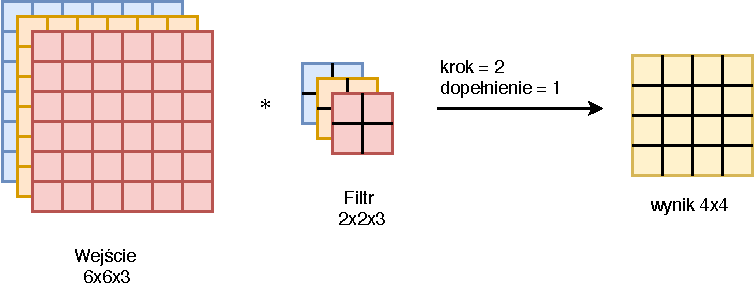
\includegraphics[scale=0.8]{resources/cnn/splot_w_cnn.pdf}}
\caption{Przykładowa operacja splotu wykonywana między dwiema warstwami sieci \textit{CNN}.}
\label{fig:splot}
\end{figure}

Operację wykonaną pomiędzy pojedynczą warstwą wejściową a odpowiadającym jej filtrem można zapisać:

niech: \(k = \left\lfloor \frac{n + 2p}{s} \right\rfloor\), \(k\ \in Z\), proponuję następujący wzór:

\[\sum_{q = 0}^{n_{w}}{\sum_{r = 0}^{k}{\sum_{l = 0}^{k}\sum_{i = 0}^{n_{g} - 1}{\sum_{j = 0}^{n_{g} - 1}{\rho\lbrack f_{q}\left( rs + i,ls + j \right) g_{q}\left( i,j \right) + b\rbrack}}}}, \tag{9}\]

gdzie:

\begin{itemize}
\item
  \(n_{w}\) -- wielkość trzeciego wymiaru wejściowej macierzy,
\item
  \(n\) -- wymiar wejściowej macierzy kwadratowej, w tym przypadku równy 6,
\item
  \(p\) -- dopełnienie, wymiar dodatkowej „obwódki'' wokół oryginalnego
  obrazu w celu wyeliminowania tzw. problemu brzegu; w tym przypadku
  równe 1.
\item
  \(s\) -- krok, z którym dopasowujemy filtr na macierz wejściową, w tym
  wypadku równy 2, to znaczy macierz filtra jest aplikowana co dwa
  elementy w pionie i poziomie (każdy piksel jest zakryty wyłącznie
  raz),
\item
  \(n_{g}\)- wymiar macierzy filtra,
\item
  \(f_{q}(i,j)\) -- funkcja reprezentująca wartości macierzy wejściowej
  warstwy \(q\),
\item
  \(g_{q}(i,j)\) -- funkcja reprezentująca wartości macierzy filtra
  warstwy \(q\),
\item
  \(\rho\) - funkcja aktywacji,
\item
  \(b\) -- bias, reprezentuje wartość neuronu gdy wszystkie aktywacje na jego wejściu są równe zero. Dokładna jego wartość jest ustalana razem z wagami podczas propagacji wstecznej,
\item
  \(k\) -- krok z jakim aplikowany jest filter na obrazie.
\end{itemize}

Wzór zaproponowany powyżej jest analogiczny do gęstego modelu wzoru na
propagację w przód \(z^{\lbrack l\rbrack} = w^{\lbrack l\rbrack}a^{\lbrack l - 1\rbrack} + b^{\lbrack l\rbrack},\ \ a^{\lbrack l\rbrack} = \rho(z_{n}^{\lbrack l\rbrack})\), jeżeli traktować \(w\), \(a\) i \(b\) jak macierze, a \(\rho\) jako operację działającą na każdym z elementów macierzy z osobna.

Uzyskane tym sposobem macierze wynikowe oraz wagowe są wielokrotnie mniejsze, kosztem tego, że te same wagi są ustalane przy pomocy różnych części obrazu. Można za to wprowadzić wiele różnych zestawów filtrów. Każdy z nich może nauczyć się wykrywać inne zależności w obrazie np. jeden może odpowiadać za wykrywanie krawędzi w pionie, inny w poziomie. W tym wypadku każdy z tych filtrów miałby wymiary 2\(\times\)2\(\times\)3. Stosując wiele różnych filtrów na raz uzyskujemy wielowymiarowy wynik
a wymiar trójwymiarowej macierzy wynikowej wynosi wtedy:
\[n_{x} \times n_{y} \times n_{z}, \tag{10}\]
gdzie \(n_{x}\) = ­­\(n_{y}\)=
\(\left\lfloor \frac{n + 2p - n_{f}}{s} \right\rfloor + 1\), \(n,\ p,\ s\)
są zgodne z opisem wyżej, \(n_{f}\ \)to wymiar macierzy kwadratowej
filtra a \(n_{z}\) -- to liczba użytych filtrów wielkości
\(n_{f} \times n_{f} \times n_{c}\), gdzie \(n_{c}\) to liczba kanałów poprzedniej warstwy.

Należy jednocześnie nadmienić, że filtry nie muszą być stosowane tylko na danych wejściowych. Wynik konwolucji może i często jest, przekazywany do głębszych warstw, gdzie uczone są filtry pracujące na wynikach warstw poprzednich. O wizualizacji tego, czego się te filtry nauczyły, będzie dalej w tej pracy.

\subsection{Warstwy łączące}

Warstwy łączące (ang. \textit{pooling layers}) są często wykorzystywane w celu zmniejszania wymiarów warstwy sieci CNN. Do najpopularniejszej należy zdecydowanie tzw. \textit{max pooling}. Polega na tym, że z obszaru w macierzy reprezentującej wartości danej warstwy w sieci konwolucyjnej wybieramy element z najwyższą wartością. Przykład operacji \textit{maxpool} przedstawia rysunek \ref{fig:maxpool}.

\begin{figure}[ht]
\centerline{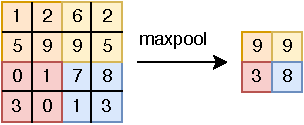
\includegraphics[scale=1]{resources/cnn/maxpool.pdf}}
\caption{Zasada działania \textit{maxpool} dla macierzy \(4 \times 4\) przy użycia filtra \(2 \times 2\), bez dopełnienia i z krokiem \(s = 2\).}
\label{fig:maxpool}
\end{figure}

Istnieje jeszcze wariacja sumująca wszystkie wartości z obszaru (ang. \textit{sum pooling}) i licząca średnią z obszaru (ang. \textit{avg pooling}). Zasady odnośnie liczenia wielkości macierzy wynikowej dotyczącą każdego z wariantów \textit{poolingu} i są analogiczne jak w przypadku obliczania splotu, z tym wyjątkiem, że \textit{pooling} stosowany jest do każdej z warstw osobno i nie wpływa na wielkość trzeciego wymiaru macierzy wynikowej.

Popularnym schematem jest stawianie warstwy \textit{poolingowej} zaraz po warstwie konwolucyjnej (wraz z wykonaniem aktywacji na wyniku). Warstwy \textit{splot-pooling} często są łączone ze sobą w różnych wariantach architektury sieci \textit{CNN}.

\section{Przykład sieci konwolucyjnej LeNet-5}
\label{lenet5}

\subsection{Schemat sieci LeNet-5}

Przy użyciu splotu, warstw łączących i sieci gęsto połączonych, można zaprezentować kompletny model sieci konwolucyjnej. Posłużę się przykładem klasycznej sieci nazwanej LeNet-5 \cite{lenetpaper}. Oryginalnie służyła do rozpoznawania odręcznie pisanego pisma.
Schemat sieci LeNet-5 przedstawia rysunek \ref{fig:lenet5}.

\begin{figure}[ht]
\centerline{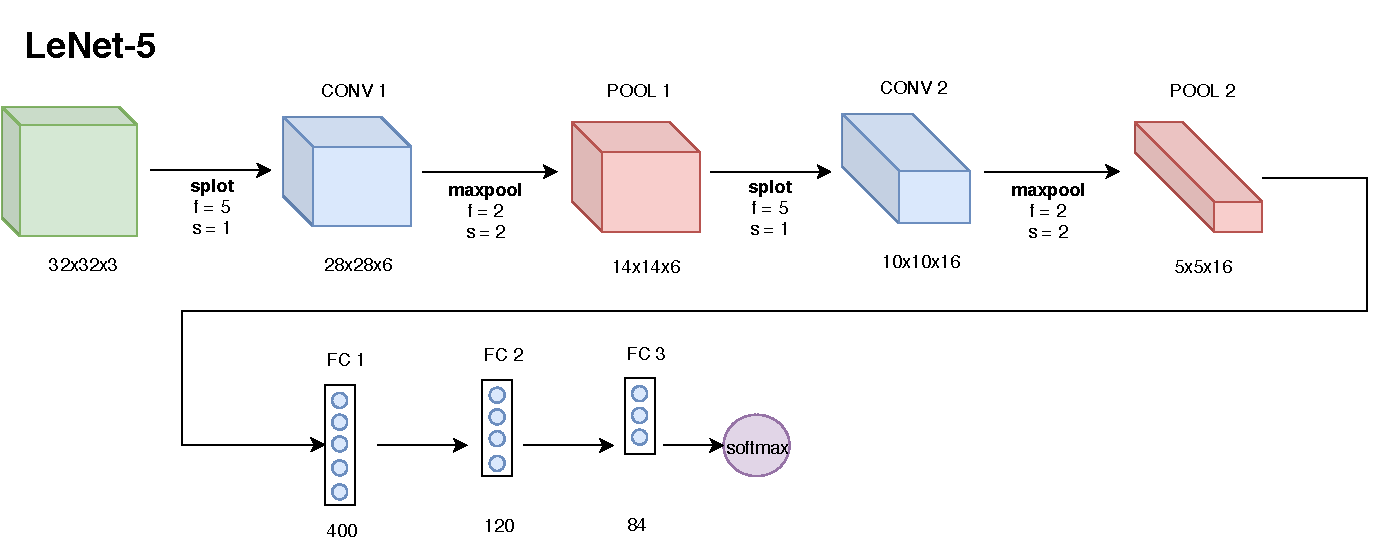
\includegraphics[scale=0.65]{resources/cnn/lenet5.pdf}}
\caption{Schemat sieci konwolucyjnej LeNet-5. Jako \(s\) oznaczono krok konwolucji a \(f\) to wymiar macierzy kwadratowych składających się na filtr.}
\label{fig:lenet5}
\end{figure}

Przyjmuje ona na wejściu obrazki o wymiarach 32\(\times\)32 pikseli z trzema kanałami (RGB), stosuje operacje splotu przy użyciu 6 filtrów o wymiarach 5\(\times\)5\(\times\)3 dając, zgodnie ze wzorem, wynik o wymiarach 28\(\times\)28\(\times\)6.
Do tak uzyskanych macierzy wprowadzany jest element nieliniowości przy pomocy funkcji aktywacji, w tym przypadku tangens hiperboliczny.
Następnie stosowana jest warstwa \textit{maxpool} o wymiarze filtra 2\(\times\)2\(\times\)6. Tak uzyskany wynik trafia na splot
tym razem 16 filtrów 5\(\times\)5\(\times\)6 i \textit{maxpool} 2\(\times\)2\(\times\)16. Następnie przekazywany jest do w pełni połączonej sieci neuronowej, trójwarstwowej, posiadającej 400, 120 i 84 węzły na kolejnych warstwach. W wersji, którą chce zaprezentować wynik uzyskam przy pomocy \textit{softmax} i będzie to 10 elementowy wektor.

\subsection{Opis implementacji sieci LeNet-5}

By zaimplementować zaproponowany model, posłużę się biblioteką do
głębokiego uczenia maszynowego -- Keras. Model będzie zaimplementowany w
języku Python (wersja 3). Z racji niewielkich rozmiarów sieć będzie trenowana przy pomocy procesora. Do
treningu użyję publicznie dostępnej bazy danych MNIST \cite{mnist}. Zawiera ona zbiór odręcznie pisanych cyfr wraz z przyporządkowaną wartością od 0 do 9.
Dane zostaną podzielone w
sposób, jaki został zaproponowany przez autorów tj. 60~000 przykładów
będzie użytych do treningu, a 10~000 do ewaluacji sprawności sieci.
Często pracuje się na trzech zbiorach danych: do uczenia, do regulacji
parametrów oraz do testów. W tym wypadku architektura sieci nie będzie
jednak zmieniana w trakcie treningu, więc zestaw służący do regulacji
zostanie pominięty.

Dane dostępne w postaci binarnej zostaną wczytane naraz do pamięci RAM.
Następnie wartości pikseli obrazu zostaną znormalizowane z przedziału
\({[}0, 255{]}\) do \({[}0, 1{]}\). Etykiety symbolizujące jaką cyfrę przedstawia obraz początkowo wczytywane są jako cyfra
z przedziału \({[}0, 9{]}\). W przypadku użycia \textit{softmax}, istnieje potrzeba
dostosowania ich do postaci wektora składającego się z zer i jedynek w
którym, jedynka wstawiona na odpowiedniej pozycji pokazuje jaka jest
wartość etykiety (ang. \textit{onehot vector}).

Niestety dostępne obrazy nie pasują formatem do zaproponowanej
oryginalnie sieci LeNet-5. Zamiast posiadać trzy kanały, obrazy
wejściowe są czarno białe i w wymiarach 28\(\times\)28 pikseli, więc
filtry pierwszej warstwy konwolucyjnej będą miały odpowiednio
zredukowany trzeci wymiar. By nie zmieniać zbytnio oryginalnej
architektury, obrazy zostały dopełnione przy pomocy zer na brzegach do
wymiaru 32\(\times\)32.

Sieć trenowana jest przy pomocy wariacji metody gradientu -- \textit{Adam} wspomnianej w rozdziale \ref{sec:backprob}. Użyta
funkcja kosztu została opisana w rozdziale \ref{sec:costfunction}. Gdy sieć
jest trenowana przy pomocy \textit{Adam}, dane użyte do treningu grupowane są w
mniejsze porcje (w tym przypadku 256 elementów), na których przeliczana
jest propagacja w przód i w tył naraz. Następnie, na sieci wynikowej
uczona jest następna porcja, aż do wyczerpania elementów ze zbioru
uczącego. Taki jeden obieg nazywamy \textit{epochem}. Podczas treningu tej sieci
wykonam 5 takich \textit{epochów}.

W celu uzyskania lepszej sprawności w przewidywaniach sieci,
zastosowałem w implementacji, nie opisane do tej pory praktyki
zapobiegające przeuczeniu sieci tzw. \textit{dropout} i normalizację porcji
(ang. \textit{batch normalization}). Dropout, losowo \textit{wyłącza} poszczególne
neurony podczas uczenia, wymuszając równomierne rozłożenie
odpowiedzialności za wykrywanie poszczególnych cech zbioru danych. \textit{Batch
normalization} natomiast skaluje wagi warstw ukrytych tak, by mediana i
odchylenie standardowe nie zmieniały się zbyt drastycznie. Daje to
pozytywne efekty dla czasu treningu sieci i w pewnym stopniu, tak samo
jak \textit{dropout}, normalizuje wagi
sieci.

\subsection{Implementacja modelu przy pomocy \textit{Keras}}

Ten niewielki model jest idealnym przykładem, w jaki sposób modeluje się sieci neuronowe przy pomocy Kerasa. 
Kod do wczytywania danych został pominięty, ponieważ nie jest istotny z punktu widzenia treningu. 
Po wczytaniu danych, obrazy użyte do treningu są dopełniane do wielkości 32\(\times\)32 przy pomocy metody \textit{ZeroPadding2D}, 
następnie przy pomocy \textit{Conv2D} definiuję warstwę konwolucyjną, normalizuję jej wagi przy pomocy \textit{BatchNormalization} i 
aktywuję przy pomocy tangensa hiperbolicznego. Następnie stosuję warstwę \textit{MaxPooling2D}, analogiczne warstwy 
\textit{Conv2D} oraz \textit{BatchNormalization} i całość wprowadzam do warstw gęstej sieci (warstwy \textit{Dense}), stosując uprzednio dwa razy \textit{Dropout}.

\begin{lstlisting}[language=Python, caption={Model sieci LeNet-5 w Keras.}, label={lst:lenet5keras}, captionpos=b]
#loading the dataset
train_labels, test_labels, train_images, test_images, 
              train_images_orig, test_images_orig = loadTrainingData();
## model fitting below ##
X_input = Input((28, 28, 1))
# Padding to the 32x32
X = ZeroPadding2D((4, 4))(X_input)
# CONV -> BN -> RELU
X = Conv2D(6, (5, 5), strides = (1, 1), name = 'conv0')(X)
X = BatchNormalization(axis = 3, name = 'bn0')(X)
X = Activation('tanh')(X)
# MAXPOOL
X = MaxPooling2D((2, 2), name='max_pool_1', strides=2)(X)
# CONV -> BN -> RELU
X = Conv2D(16, (5, 5), strides = (1, 1), name = 'conv1')(X)
X = BatchNormalization(axis = 3, name = 'bn1')(X)
X = Dropout(0.4, name='drop_1')(X)
X = Dropout(0.3, name="drop_2")(X)
X = Dense(400, activation='tanh', name='fc_in')(X)
X = Dense(120, activation='tanh', name='fc_mid')(X)
X = Dense(84, activation='tanh', name='fc_out')(X)
X = Dense(10, activation='softmax', name='fc_softmax')(X)
# Create model
model = Model(inputs = X_input, outputs = X, name='ResNet-5')
model.compile(optimizer="Adam", 
              loss="binary_crossentropy", metrics=["accuracy"])
# Fit the model
model.fit(x=train_images, y=train_labels, epochs=5, batch_size=256)
# Evaluate
preds = model.evaluate(x = test_images, y = test_labels)
print ("Loss = " + str(preds[0]))
print ("Test Accuracy = " + str(preds[1]))
\end{lstlisting}

Model zdefiniowany przy pomocy klasy \textit{Model}, trenowany jest przy pomocy funkcji optymalizującej \textit{Adam} przy użyciu funkcji 
kosztu \text{binary crossentropy} zdefiniowanych przy pomocy metody \textit{compile}. Trening modelu zaczyna się po wywołaniu metody \textit{fit}, przyjmującej dane, na których ma być wytrenowana.
Metoda \textit{evaluate} testuje skuteczność modelu na danych testowych. Wynik treningu sieci LeNet-5 przedstawia rysunek \ref{fig:lenet5-training}.

\begin{figure}[ht]
\centerline{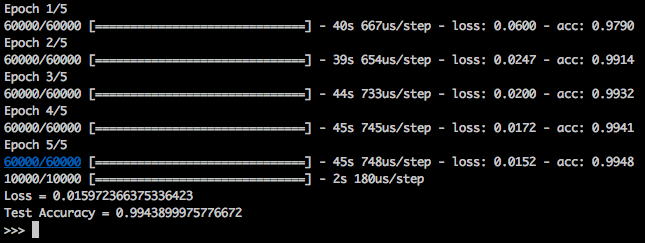
\includegraphics[scale=0.5]{resources/training_lenet5.png}}
\caption{Wynik treningu sieci LeNet-5.}
\label{fig:lenet5-training}
\end{figure}

Trening trwał niecałe 4 minuty i uzyskał skuteczność powyżej 99\%, co jest bardzo zadawalającym wynikiem. Przykładowy obraz ze zbioru treningowego pokazuje rysunek \ref{fig:lenet5-digit} a odpowiedź modelu na pytanie jaka to cyfra znajduje się na rysunku \ref{fig:lenet5-response}.

\begin{figure}[ht]
\centerline{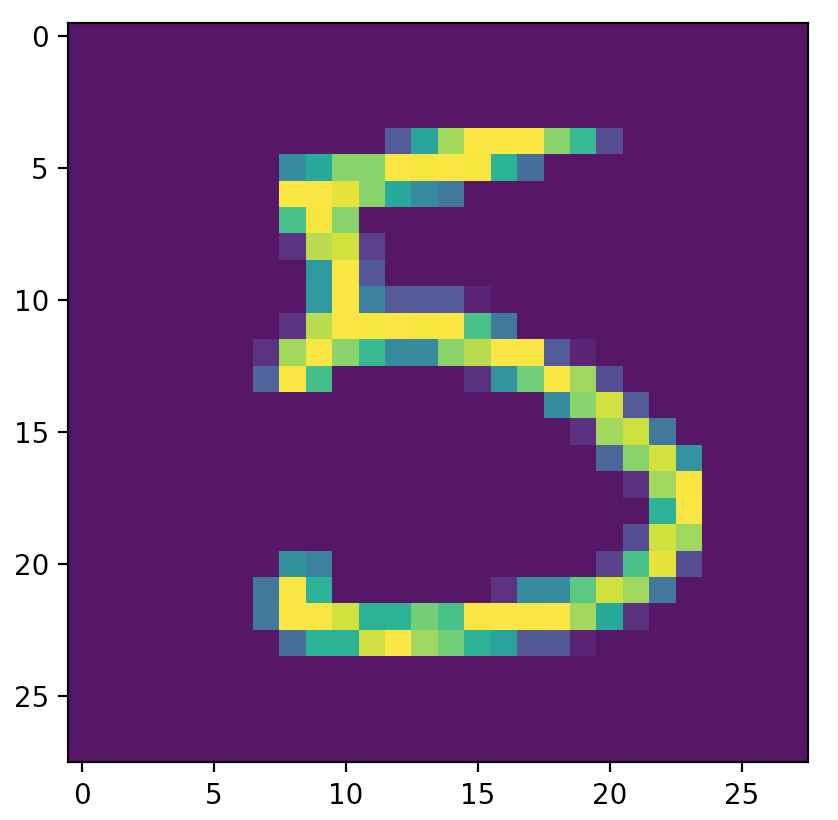
\includegraphics[scale=0.5]{resources/example_digit_lenet5.png}}
\caption{Przykładowy obraz ze zbioru testowego.}
\label{fig:lenet5-digit}
\end{figure}

\begin{figure}[ht]
\centerline{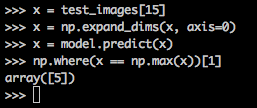
\includegraphics[scale=0.5]{resources/example_digit_lenet5_response.png}}
\caption{Odpowiedź modelu na pytanie, jaką cyfrę rozpoznaje.}
\label{fig:lenet5-response}
\end{figure}

\label{lenet-wiz}
\subsection{Wizualizacja neuronów warstw konwolucyjnych sieci LeNet-5.}
Mając do dyspozycji wytrenowany model, można przystąpić do próby wizualizacji tego, czego nauczyła się sieć. Przy modelu tak płytkim jak LeNet-5 uzyskane odpowiedzi powinny być mniej imponujące wizualnie, ale przez to łatwiejsze w interpretacji.

\subsubsection{Wizualizacja poprzez wyświetlenie wag warstw konwolucyjnych.}
Pierwszy ze sposobów, który zaprezentuję będzie też najprostszy koncepcyjnie. Wyrysowanie filtrów warstw konwolucyjnych powinno dać ogólny zarys tego, jakie cechy obrazu (gradient, linie poziome/pionowe/ukośne) były brane pod uwagę przez sieć. W celu łatwiejszej intrepretacji zestawię ze sobą filtry 5\(\times\)5 oryginalnie występujące w sieci LeNet-5 z wariacją sieci wytrenowanej na filtrach 3\(\times\)3, którą wytrenowałem tylko po to, by mieć punkt odniesienia do filtrów
klasycznie używanych w analizie obrazu.
Wizualizację uzyskanych filtrów pokazuje rysunek \ref{fig:lenet5-response2}.

\begin{figure}[ht]
\centerline{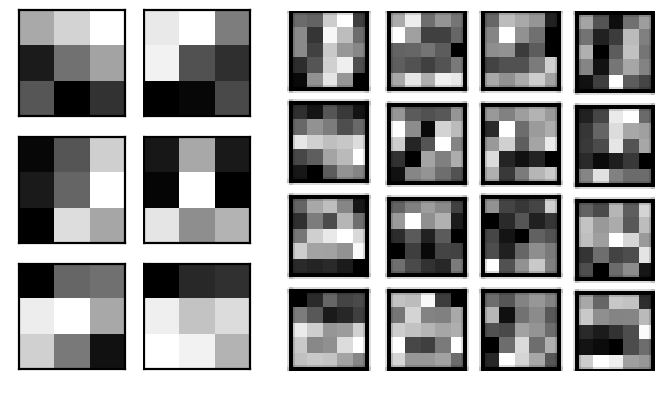
\includegraphics[scale=0.5]{resources/plot_filtry.png}}
\caption{Wizualizacja filtrów sieci LeNet-5. Od lewej filtry warstwy pierwszej wersji zmodyfikowanej 3\(\times\)3. Z prawej filtry warstwy drugiej wersji oryginalnej.}
\label{fig:lenet5-response2}
\end{figure}

Na filtrach 3\(\times\)3 widać tendencję w wykrywaniu krawędzi pionowych, poziomych i ukośnych. Dodatkowo duży nacisk położony jest na wykrywanie gradientu po skosie (dwa pierwsze filtry od góry i dwa ostatnie od dołu).
Widoczne jest, że macierze filtrów odbiegają trochę wartościami od klasycznie używanych macierzy w analizie obrazów. Mogło być to spowodowane przedewszystkim charakterem używanego zbioru danych, sieć mogła dostosować używane filtry by te pasowały jak najbardziej do danych wejściowych. Dodatkowo, użyte dopełnienie z \(28\) do \(32\) pikseli nie było obojętne na uzyskane wartości w macierzach.

W przypadku filtrów 5\(\times\)5 kształty, które próbuje dopasować sieć robią się bardziej skomplikowane, przez co trudniejsze w interpretacji. Podobnie jak w przypadku filtrów warstwy pierwszej, można znaleźć filtry szukające ukośnych gradientów oraz linii w pionie i poziomie, ale oprócz tego znajdują się tu filtry, które intrepretowałbym jako elementy strukturalne próbujące dopasować się do konkretnych kształtów występujących w poszczególnych elementach. Należy jednak podkreślić, że
wyświetlone filtry 5\(\times\)5 operują na wyniku konwolucji i \textit{maxpoolingu} warstwy pierwszej -- są przez to trudne w intrepretacji.

Wniosek jest taki, że tym wypadku najprostsze rozwiązanie nie jest najlepsze. Nie będę więc dalej analizował tej metody ani stosował jej dla modeli o większej złożoności, bo im głębszą warstwę sieci wybiorę tym trudniejsze w intrepretacji będą wyniki.

\subsubsection{Wizualizacja poprzez mapy cech.}
Mapy cech czy inaczej mapy aktywacji, wizualizują rezultat zastosowania filtrów na danych wejściowych -- np. obrazu wejściowego czy innej mapy cech. Przykładowo, dla danego obrazu można wyrysować jakie, konkretnie jego cechy zostały wyszczególnione przez warstwę sieci CNN. 
By uzyskać mapę cech dla danego obrazu, należy zmodyfikować model w taki sposób, by jego warstwą wyjściową była ta warstwa konwolucyjna, której cechy chcemy uzyskać. Przykładowe mapy cech pokazuje rysunek \ref{fig:lenet5-mapy-aktywacji-l1} i \ref{fig:lenet5-mapy-aktywacji-l2}.

\begin{lstlisting}[language=Python, caption={Uzyskiwanie mapy aktywacji dla danego modelu i obrazu w Keras.}, label={lst:lenet5keras-mapy}, captionpos=b]
img = np.expand_dims(img, axis=0)
vmodel = Model(inputs=model.inputs, outputs=model.layers[layer_no].output)
feature_maps = vmodel.predict(img)
\end{lstlisting}

W ogólności, warstwy bliżej źródła danych powinny zawierać informacje o dużej ilości szczegółów, a warstwy głębsze, wykrywać cechy bardziej ogólne. I tak, 
dla pierwszej warstwy konwolucyjnej sieci LeNet-5 wyrysowane cechy dla przykładu z każdej klas bardzo mocno przypominają oryginalne obrazy. Dostrzegalne różnice pomiędzy warstwami polegają na dostrzeganiu innego ,,konturu'' obrazu każda z warstw akcentuje inny jego rodzaj, przez co liczby dają iluzję bycia ,,oświetlonymi'' z różnych stron.
Zgadza się to z obserwacją poczynioną w przypadku analizy wartości filtrów. Dodatkowo, każda aktywacja różni się trochę kolorem tła co nasuwa logiczny wniosek, że aktywacja nie jest zależna od tła otoczenia (choć prawdopodobnie niejednolite tło mogłoby negatywnie wpłynąć na wydajność sieci).

\begin{figure}[ht]
\centerline{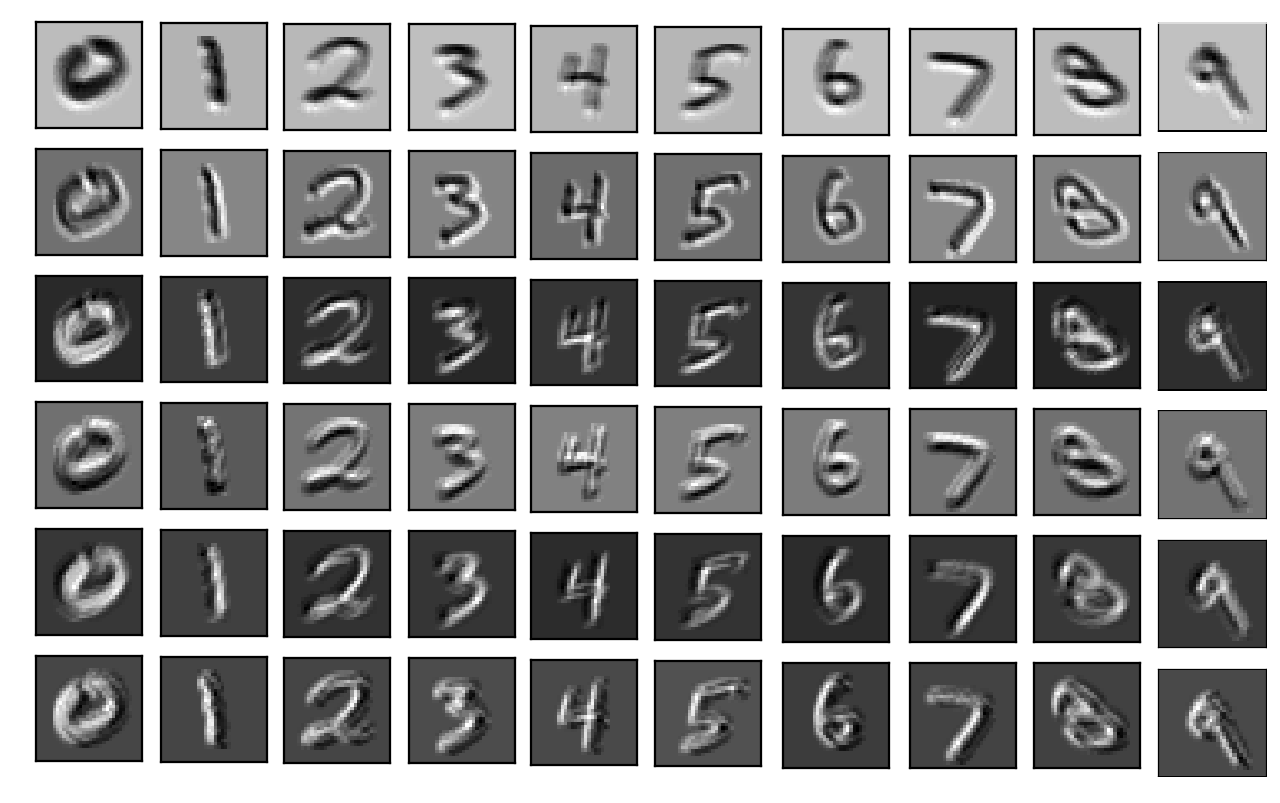
\includegraphics[scale=0.25]{resources/first_layer_gd_lenet.png}}
\caption{Mapy aktywacji dla 6 filtrów warstwy pierwszej, przy użyciu przykładu dla każdej z klas. Filtry użyte do aktywacji ustawione są w rzędach tak, że indeks rzędu odpowiada numerowi filtra. Kolejne kolumny odpowiadają użytej klasie. }
\label{fig:lenet5-mapy-aktywacji-l1}
\end{figure}

Sytuacja robi się jeszcze ciekawsza w przypadku warstwy drugiej. Tam jest już 16 filtrów, więc nie zostaną zaprezentowane dla każdej z klas z osobna. Niemniej jednak, sam wynik dla pojdynczej klasy jest w stanie wiele powiedzieć na temat branych pod uwagę cech.

\begin{figure}[ht]
\centerline{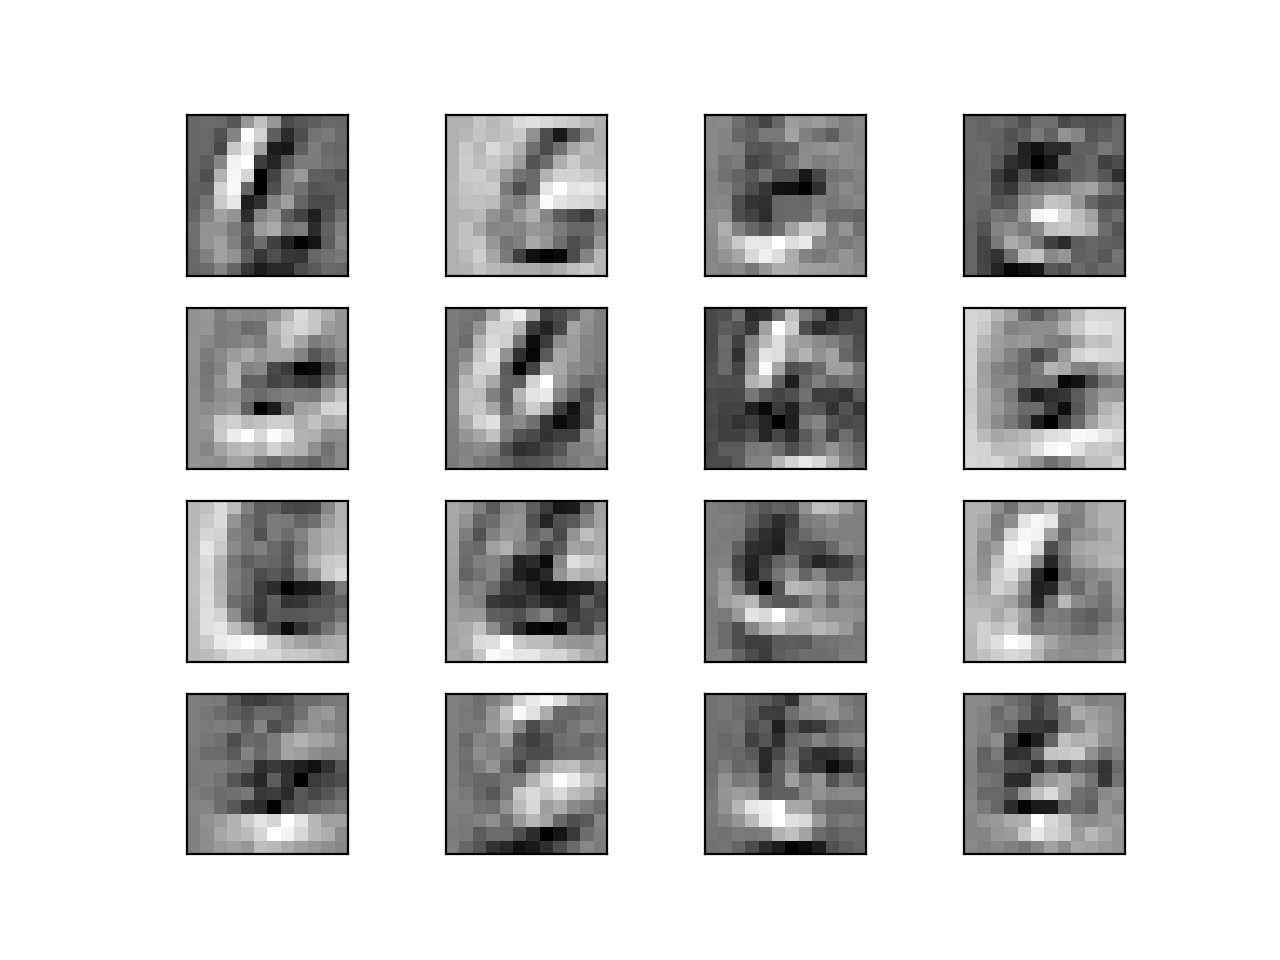
\includegraphics[scale=0.75]{resources/second_layer_gd_lenet.png}}
\caption{Mapy aktywacji dla 16 filtrów warstwy drugiej, przy użyciu przykładowej reprezentacji liczby 6.}
\label{fig:lenet5-mapy-aktywacji-l2}
\end{figure}

Uzyskane aktywacje wciąż przypominają oryginalną szóstkę, lecz tym razem, zgodnie z oczekiwaniami, cechy są bardziej zgeneralizowane.
Wyraźnie widać skupienie filtrów na dolnej ,,pętli'' szóstki oraz na tym, by posiadała odpowiednie łuki na brzegach (wyraźnie zarysowany jest tam gradient, widoczny szczególnie na filtrach w ostatnim rzędzie).

Niestety sieć LeNet-5 jest na tyle płytka, a zestaw odręcznie pisanych cyfr na tyle mało skomplikowany, że nie uda mi się przy ich pomocy wyekstrahować bardziej złożonych wzorów. W tym celu będę musiał posłużyć się bardziej złożonym modelem -- siecią VGG-19. 
